\section{Emulsion stability and microstructures}

When two partially miscible fluids are mixed together, they will have the tendency to coalesce into two distinct phases as they attempt to minimize 
the thermodynamic penalty accrued from the formation of an interface. To prevent this coalescence process, conventionally small molecule surfactants 
are utilized. The most famous example of this class of material is soap which emulsifies dirt into droplets suspended in water through mechanical action. 
Surfactants function through reducing the surface tension between the droplet, known as the dispersed phase, and the bulk fluid, known as the continuous 
phase. Surfactants function through reducing the surface tension between dispersed and continuous phases, reducing the energy penalty owed from formation 
of an interface.

The existence of particle stabilized emulsions has been known for more than a century now, after Pickering and Ramsden independently identified dispersed 
droplets of oil within a water matrix after vigorous stirring of an oil, water and particle mixture. 
\textcolor{blue}{10.1098/rspl.1903.0034, http://pubs.rsc.org/en/content/articlelanding/1907/ct/ct9079102001} Unlike surfactants, 
particles act as emulsion stabilizers through the reduction of contact between dispersed and continuous phases as they adsorb into 
the interface between phases. The Pieranski model derived from observations of \textcolor{blue}{insert derivation of pieranski model} 
and is used to determine the adsorption energy of a particle at an interface. It is defined as $G_{ads} = \sigma A_{rm} (1 - \cos{\theta_c})^2$, where $G_{ads}$ 
is the free energy reduction from a particle adsorption, $\sigma$ is the surface tension between the partially miscible fluids, $\theta_c$ is the contact angle 
of the particle. The particles can be considered to be irreversibly adsorb even for nanoparticles, and for particles larger than 100nm, the adsorption energy 
is so great that thermal fluctuations at the interface can be considered to have no effect. \textcolor{blue}{https://doi.org/10.1063/1.3618553} 

After their discovery, interest in particle stabilized emulsions became minimal. However, increased interest in them has resurfaced since the 1980s owing to 
their applications in food science. One such example is fat crystals stabilizing water droplets in oil to create margarine. Particle stabilization has also 
been of interest owing to their lower toxicity and greater ease of sustainable sourcing through the usage of cellulose or chitin particles. \
textcolor{blue}{https://www.tandfonline.com/doi/full/10.1080/14686996.2017.1401423, 10.1021/acs.biomac.6b00144, 10.1021/acs.langmuir.7b03959} 
Additionally, chemical surfactants can be toxic to aquatic life, acting as a xeno-hormone and interfering with their reproduction. 
\textcolor{blue}{https://www.sciencedirect.com/science/article/pii/S0304389420302879, https://www.sciencedirect.com/science/article/pii/S014765131530172X} 

Compared to emulsions stabilized using surfactants, particle stabilized emulsions offer greater resistance to coarsening, resulting in increased interest in 
them once again. The microstructure properties of particle stabilized emulsions were explored in the early 2000s by Lumsdon and Binks among many others. They 
observed that the radius of emulsion droplets, $R_e \propto \frac{\phi_w}{\phi_p}$, where $\phi_w$ and $\phi_p$ are volume fractions of water and particles 
respectively. \cite{binks_pickering_2001} They also identified that there were other techniques to modify the microstructure of a Pickering Emulsion 
such as concentration of fluids and particle wettability. Neutrally wetting particles do not impart a preferential curvature to the interface. When 
using non-neutrally wetting particles, bridged droplets, capillary aggregates and other non droplet microstructures can be observed. Bijels, are synthesized 
in a system using equal volume fraction of fluids and neutrally wetting particles, thus facilitating the formation of tortuous, co-continuous domains. 

Bijels are synthesized in systems which have roughly equal fluid volume fractions and neutrally wetting particles so as to not impose preferential 
curvature on the interface. \cite{stratford_colloidal_2005, herzig_bicontinuous_2007, lee_bicontinuous_2010, jansen_bijels_2011, velankar_non-equilibrium_2015} 
Reeves et al. demonstrated that bijels stabilized with nanoparticles are more stable than those with microparticles due to better mechanical properties and 
interface coverage. \cite{reeves_particle-size_2015}  Additionally, research by Jansen, Harting, and Hijnen et al. showed that the bijel domain size 
$L \propto \frac{1}{\phi_p}$ for both rod-like and spherical particles. Although the pre-factor is dependent upon the particle geometry, this feature 
has been seen with many other particle shapes as well. \cite{hijnen_bijels_2015, madivala_exploiting_2009, gunther_timescales_2014, daware_emulsions_2015, 
loudet_capillary_2005, cheng_shape-anisotropic_2013}

% While bijels are a relatively new material class, much work has been conducted to elucidate the underlying mechanisms controlling their stability, microstructure and rheology. Many studies focus on how the particle properties play important roles in tuning the properties of bijels. This section will cover a brief overview and summary of literature on the working principle behind particle surfactants, the effect of size and concentration of particles, anisotropic particles in particle stabilized emulsions, microstructure control in various bijel synthesis techniques, stimuli response in bijels and bijel rheology. 

\begin{figure}
    \centering
    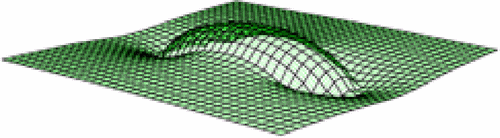
\includegraphics[scale = 0.5]{figures/literature_review/interfacial_curvature.png}
    \caption{Quadropolar capillary interactions around prolate ellipsoidal particles caused by interfacial deformations around the particle. 
    \cite{loudet_capillary_2005} Reproduced from Loudet et al. with license number RNP/25/FEB/088185}
    \label{fig:anisotropic_particle_interface}
\end{figure}

\section{Particle shape anisotropy and synthesis techniques}

In the past decade, methods to synthesize particles which have anisotropic geometry and chemistry have increased in number and scope. Synthesis techniques vary 
depending on the type of particle shape desired. Ellipsoids can be easily created by mechanical deformation of polymer spheres. Dumbbell shaped particles can be 
synthesized using microfluidic devices or emulsion templating. Square particles can be generated using crystallization of material. \cite{morgan_understanding_2013} 
These variety of techniques mean that particle geometry is no longer as constraint when investigating prospective particle stabilizers of bijels. 
\textcolor{blue}{https://onlinelibrary.wiley.com/doi/10.1002/smll.201600877}

Anisotropic particles have shape dependent properties owing to their induction of multipolar interactions by deforming the interface to ensure the mean 
curvature is 0,  fulfilling the Young-Laplace equation shown in Figure \ref{fig:anisotropic_particle_interface}. \cite{loudet_capillary_2005, 
cheng_shape-anisotropic_2013} Using this property has enabled directed assembly and migration through modified capillary forces. 
\cite{cavallaro_curvature-driven_2011, read_dimerization_2020, sharifi-mood_curvature_2015} 

Anisotropic particles have also been shown to exhibit natural liquid crystal like behaviour as shown using Onsager theory. 

When stabilizing bijels, ellipsoidal particles offer greater stability than spherical ones due to their larger cross-sectional area to volume ratio, 
as shown by Günther et al. and Hijnen et al. \cite{gunther_timescales_2014, hijnen_bijels_2015} This results in additional domain coarsening timescales 
from particle re-orientation and increased mechanical rigidity, enhancing the stability of emulsions with ellipsoidal particles, as evidenced in rheological 
studies. \cite{gunther_timescales_2014, daware_emulsions_2015, witt_bijel_2013} It has also been shown that particle shape changes how and when jamming occurs. 
Using graphene plate like particles, it was shown that the plate like particles can have their own elasticity to them, affecting when jamming occurs. 
\textcolor{blue}{https://doi.org/10.1039/C3MH00047H, https://pubs.acs.org/doi/10.1021/la402436w}

Control over the orientation of ellipsoidal particles at interfaces balances interfacial capillary and magnetic field forces. 
\cite{bresme_orientational_2007, davies_assembling_2014} Theory and simulations indicate a critical field strength above which particle orientation 
is dominated by the applied field. \cite{bresme_orientational_2007, davies_assembling_2014} Experiments and simulations have found that steric interactions, 
influenced by orientation and interfacial arrangements significantly influence the free energy of particle assemblies, highlighting the complex interplay 
between these forces. \cite{morgan_understanding_2013, newton_influence_2014, newton_capillary_2018}

% The adsorption process is affected by the shape of particles used as they pack differently onto the interface \cite{hijnen_bijels_2015, daware_emulsions_2015,carmack_diverse_2017}. It has also been suggested that adsorption dynamics of ellipsoidal particles at liquid interfaces are driven completely by viscous forces even if the timescales of adsorption are driven by particle properties \cite{Coertjens2017}. Some guiding equations to calculate the interfacial area of an ellipsoidal particle are provided \cite{gunther_timescales_2014, Davies2014}.

\section{Bijel synthesis techniques}

Bijels were first synthesized using Thermally Induced Phase Separation (TIPS). \cite{herzig_bicontinuous_2007, lee_bicontinuous_2010, bai_dynamics_2015} 
First, a small molecule or polymer blend with a critical point, named the casting mixture, is identified and prepared with a composition corresponding to 
that of the critical point. Next, the casting mixture is blended with particle surfactants while still in a single phase. Once the particles are distributed 
homogenously in the casting mixture, phase separation is initiated in the casting mixture through changing the temperature such that it is in the two-phase region. 
Through ensuring the composition is that of the critical point, the casting mixture undergoes spinodal decomposition without any nucleation and growth. 

TIPS allows for batch synthesis of bijels in research labs. However to make bijels industrially relevant, a continuous process which also facilitates the 
synthesis of multiple form factors of bijels for various applications. Solvent Transfer Induced Phase Separation (STrIPS) was proposed as a means to do just this. 
A casting mixture composed of two fluids, a co-solvent, particles and a surfactant is prepared. The fluids will constitute the bijel while the co-solvent will 
diffuse out of the bijel to initiate phase separation. The surfactant is present to ensure that the bijel remains stable against Marangoni pressure. The casting 
mixture if extruded into a bath of non-solvent that is not miscible with the bijel constituents but is miscible with the co-solvent. Diffusion of co-solvent 
initiates phase separation and synthesis of the bijel. The concentration of surfactant and the flow rate of the casting mixture control the obtained microstructure. 

\textcolor{blue}{Description of VIPS}

\textcolor{blue}{Description of homogenization}

\textcolor{blue}{Description of liquid in liquid printing}

% STrIPS, shown in Figure \ref{fig:strips}, and many other fabrication techniques require fine control over the composition of the casting mixture for the technique to function and to control the obtained microstructure. \cite{haase_continuous_2015, amirfattahi_fabrication_2024, sprockel_fabrication_2023} In homogenization, the applied shear of mixing initiates coalescence of droplets in a controlled way, leading to formation of the bijel. \cite{cai_bijels_2017} In both synthesis strategies, the rheology of a proposed casting mixture is therefore essential to understand to explore what other casting mixtures can be utilized in these fabrication techniques. Microstructure control has also been achieved when using TIPS by controlling the concentration of particles at different heights, creating a gradient of pore sizes in the final bijel. \cite{french_bicontinuous_2022} Looking to the current state of stimuli response in bijels, 

% \begin{wrapfigure}{r}{7cm}
% \caption{Schematic of a bijel with hard-sphere particles undergoing shear, demonstrating migration and detachment of particles at the interface. \cite{bonaccorso_shear_2020}}
% \label{wrap-fig:bijel_under_shear}
% 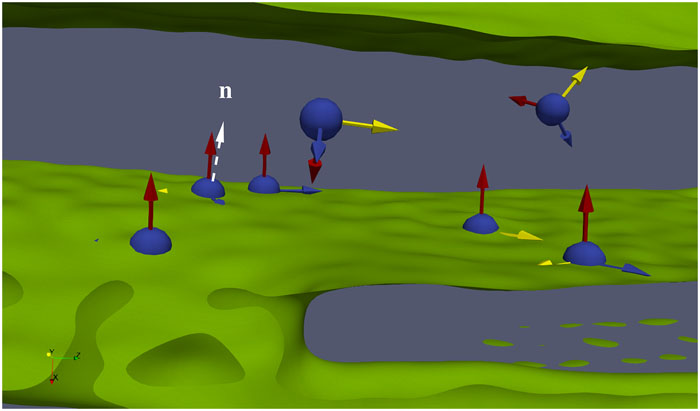
\includegraphics[width=7cm]{figures/literature_review/bijel_under_shear.jpeg}
% \end{wrapfigure}

\section{Rheological models and shear response of bijels}

\begin{figure}
    \centering
    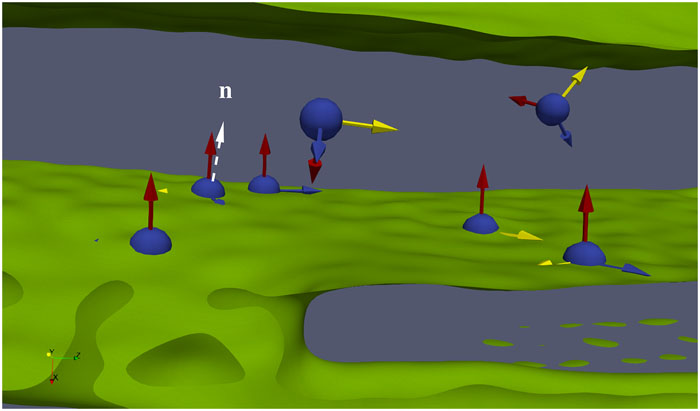
\includegraphics[scale = 2]{figures/literature_review/bijel_under_shear.jpeg}
    \caption{Schematic of a bijel with hard-sphere particles undergoing shear, demonstrating migration and detachment of particles at the interface. 
    \cite{bonaccorso_shear_2020}}
    \label{fig:bijel_under_shear}
\end{figure}

Studies into bijel rheology have shown the characteristics of a gel when the
storage modulus exceeds the loss modulus. \cite{lee_making_2013, bai_dynamics_2015} Ching and Mohraz also demonstrated that the rheological behaviour of a 
bijel most closely resembles a 2D colloidal glass that was percolating in 3D space by comparing the linear visco-elasticity of bijels with colloidal gels made 
with strongly attractive particles. \cite{ching_bijel_2022} Several key feature of glasses are that they posses a yield stress, viscoelastic behaviour and a 
glass transition point. \cite{pham_yielding_2008, weeks_introduction_2017} Yield stress is the stress imparted when the particle monolayer is irreversibly changed. \cite{pham_yielding_2008} Viscoelasticity is present when the particle monolayer has solid and a liquid like behaviour, depending upon the timescale of the applied stress. \cite{pham_yielding_2008} The glass transition point is characterized when the dynamics of the monolayer drastically slow down. \cite{weeks_introduction_2017} Figure \ref{fig:bijel_under_shear} demonstrates Bonnacorso et al.'s findings that when subjecting a bijel stabilized with hard-sphere like spherical particles to shear, the particles align to the direction of applied shear before detaching from the interface. \cite{bonaccorso_shear_2020} Looking to how particle alignment affects rheology, past work in suspension rheology has shown that colloidal systems with hard-sphere interparticle interactions undergoing constant shear demonstrate particle ordering (shear banding) in the direction of shear at moderate shear rates, causing shear thinning. \cite{vermant_flow-induced_2005, brader_nonlinear_2010} 

\textcolor{blue}{https://www.mdpi.com/2311-5521/5/3/150}

\section{Colloidal glasses}

\begin{itemize}
    \item https://pubs.acs.org/doi/10.1021/acsmacrolett.6b00826
    \item Add stuff on dynamic heterogeneity
    \begin{itemize}
        \item https://pubs.rsc.org/en/content/articlelanding/2012/sm/c2sm25267h
    \end{itemize}
    \item Add stuff on particle jamming
    \begin{itemize}
        \item https://journals.aps.org/rmp/pdf/10.1103/RevModPhys.82.2633
    \end{itemize}
    \item Add stuff on cooperatively rearranging regions
        \begin{itemize}
            \item https://doi.org/10.1038/ncomms4829
            \item https://journals.aps.org/prl/abstract/10.1103/PhysRevLett.110.188301
            \item https://journals.aps.org/prl/abstract/10.1103/PhysRevLett.107.065702
        \end{itemize}
    \item Add stuff on reentrant glass phenomena 
    \begin{itemize}
        \item https://doi.org/10.1209/0295-5075/86/58001
    \end{itemize}
\end{itemize}

\section{Stimuli response in particle stabilized emulsions}

Kim et al. found that strong magnetic fields do not significantly alter the microstructure of a bijel stabilized with spherical particles, as the particles orient 
to the field without affecting interface ordering. \cite{kim_bijels_2010} In contrast, Carmack and Millet demonstrated that polarizable fluids and particles under 
an electric field show significant microstructural changes, with particles self-assembling into chains and forming cylindrical domains parallel to the applied field, 
thus modifying the microstructure. \cite{carmack_tuning_2018}

\section{Lattice Boltzmann Method}

The Lattice Boltzmann Method (LBM) is an evolution of preceding lattice gas automata techniques, which is a discretization of the Boltzmann equation of motion for 
molecules. This means that unlike traditional CFD techniques such as FDM, VOF or level set methods, LBM is a psuedo-molecule method that tracks the evolution of a 
particle distribution function within grid cells evolved through a discretized Boltzmann equation of motion. Macroscopic variables such as fluid density and 
velocity are recovered from the particle distributions through appropriate moment integration, and the Navier Stokes equation at the incompressible limit can be 
obtained through a Chapman-Enskog expansion of the LBM. The LBM has become an attractive tool for meso-scale CFD simulations due to its ease of algorithm 
implementation, highly parallelizable nature and ease of boundary condition implementation, allowing coupling to other physically relevant systems such as 
particles with varieties of potentials, external fields and deformable bodies.

The particle distribution function described earlier is advected on a pre-constructed lattice stencil, commonly denoted as DnQm where n and m represent the 
number of dimensions and directions in the stencil. Common stencils include the D1Q5, D2Q9 and D3Q19 stencil, all of which recover mass and momentum conservation. 
For energy conservation, a higher order stencil such as D3Q27 is necessary. The D2Q9 and D3Q19 stencils have 8 and 18 populations respectively that include 
connections to nearest and next nearest neighbour points, in addition to a central rest point. 

The LBM is composed of a collision and advection step. In the advection step, the populations at each grid point are propagated to adjacent points in accordance 
with the chosen stencil. During the collision step, the particle population distribution is relaxed towards an equilibrium with a collision operator, at a 
specified relaxation rate. The collision operator can have multiple forms based on how many relaxation rates are used although the most common variant is the 
Single Relaxation Time (SRT) collision operator, more commonly known as the Bhatnagar-Gross-Krook (BGK) collision operator. Owing to its stability in low Mach 
and Reynolds numbers and simplicity of implementation, the BGK operator is often used in common particle laden flow and soft matter scenarios. 
\cite{bhatnagar_model_1954} These limitations are present owing to the implicit link between the fluid properties and the relaxation rate necessitating 
relaxation rates above 0.5, and to ensure fluid incompressibility from an equation that intrinsically simulates a compressible fluid. To get over these 
limitations, Two Relaxation Time (TRT) and Multiple Relaxation Time (MRT) operators also exist, expanding the possible application of the LBM to visco-elastic 
flows and implementation of fluctuating hydrodynamics in the LBM. 
\textcolor{blue}{https://pubs.acs.org/doi/10.1021/acsomega.3c06663, https://iopscience.iop.org/article/10.1209/epl/i2004-10542-5, https://link.aps.org/doi/10.1103/PhysRevE.82.056714}

Five primary techniques to model multicomponent or multiphase systems exist in the LBM literature. A quick review of the Shan-Chen or 
interparticle potential model  will be provided here from the perspective of a binary mixture. Additionally, the names and descriptions of 
other techniques will be described as well. The interparticle potential model or Shan-Chen model that adds a non-local density dependent force 
between two species, effectively modelling non-ideal mixing and recovering the Cahn-Hilliard equation. To alleviate the standard Shan-Chen implementations 
weaknesses of not being thermodynamically consistent and reducing the existence of spurious velocities, 

In addition to the Shan-Chen model, the color gradient model, free energy model, mean field theory model and interface tracking technique all 
allow for simulations of various types of multiphase and/or multicomponent flows. The color gradient model proposed by Rothman and Keller and 
implemented by Gunstensen et al relies upon modelling two particle distributions. These represent a binary fluid mixture with the collision step 
able to recover the hydrodynamics and non-ideal mixing dynamics. The free energy model utilizes phase field theory and constructs a free energy 
functional to recover interfacial dynamics and effects in a thermodynamically consistent manner. Often, a square gradient free energy is used for 
simplicity and ease of implementation. The mean field theory 

The non-ideal mixing dynamics are recovered during the "recoloring" step, of which the technique proposed by Latva-Kokko and Rothman is more commonly 
used for soft matter flows.

\textcolor{blue}{https://pure.tue.nl/ws/files/25832941/1404.7523.pdf}